%=====================================================================
% MundiPets — Parallel manuscript, version 2.0 (Deliverable 4 / 2B, week 17)
% Springer Nature journal template (sn-jnl.cls, v3.1 December 2024)
%
% Empirical component: APPROACH 2 of the course guide —
% automatic detection of ambiguity and smells in requirements.
%
% TEMPLATE: confirmed by the team as sn-jnl.cls (Springer Nature),
% Requirements Engineering journal. Not changing to REFSQ/llncs.cls.
%
% CORPUS: the requirements corpus was revised and expanded after the ERS
% renumbering (Nieves), from N=50 to N=61 (27 RF + 16 RNF + 9 RD + 9 RL).
% Every number in this version reflects the corpus of 61 requirements and
% the corrected, de-identified evaluator labels (Experto 1/2/3).
%
% Reference style: sn-mathphys-num (numbered).
%
% ### ESTADO DE ESTA VERSION ###
% Version 5 de 5 (COMPLETA) - aportes de: Fuertes Arraes + Mendoza Parraga
% + Gutierrez Ortega + Morales Sanchez + Nieves Sanchez. Todas las secciones
% cerradas para la entrega 2B.
%=====================================================================
\documentclass[pdflatex,sn-mathphys-num]{sn-jnl}

\usepackage{graphicx}%
\usepackage{multirow}%
\usepackage{amsmath,amssymb,amsfonts}%
\usepackage{amsthm}%
\usepackage{mathrsfs}%
\usepackage[title]{appendix}%
\usepackage{xcolor}%
\usepackage{textcomp}%
\usepackage{manyfoot}%
\usepackage{booktabs}%
\usepackage{algorithm}%
\usepackage{algorithmicx}%
\usepackage{algpseudocode}%
\usepackage{listings}%

% Visible marker for values the team must still fill in by hand.
\newcommand{\TODO}[1]{\textcolor{red}{\textbf{[TO COMPLETE: #1]}}}
% Marker for content deliberately deferred to Deliverable 4 (2B).
\newcommand{\DEFERRED}[1]{\textcolor{blue}{\textit{[Deferred to Deliverable 4 (2B): #1]}}}

\theoremstyle{thmstyleone}%
\newtheorem{theorem}{Theorem}%
\newtheorem{proposition}[theorem]{Proposition}%
\theoremstyle{thmstyletwo}%
\newtheorem{example}{Example}%
\newtheorem{remark}{Remark}%
\theoremstyle{thmstylethree}%
\newtheorem{definition}{Definition}%

\raggedbottom

\begin{document}
	
	\title[Accuracy of a requirements ambiguity detector]{Accuracy of a
		requirements ambiguity detector: case of a pet social network}
	
	\author*[1]{\fnm{Edson Daniel} \sur{Fuertes Arraes}}\email{efuertesa2@uteq.edu.ec}
	
	\author[1]{\fnm{Génesis Adriana} \sur{Gutiérrez Ortega}}\email{ggutierrezo@uteq.edu.ec}
	
	\author[1]{\fnm{Andy Johel} \sur{Mendoza Párraga}}\email{amedozap9@uteq.edu.ec}
	
	\author[1]{\fnm{Gary Alejandro} \sur{Morales Sánchez}}\email{gmoraless2@uteq.edu.ec}
	
	\author[1]{\fnm{Jimmy Samuel} \sur{Nieves Sánchez}}\email{jnievess@uteq.edu.ec}
	
	\author[1]{\fnm{Gleiston Cicerón} \sur{Guerrero Ulloa}}\email{gguerrero@uteq.edu.ec}
	
	\affil*[1]{\orgdiv{Facultad de Ciencias de la Computación},
		\orgname{Universidad Técnica Estatal de Quevedo},
		\orgaddress{\street{Av. Quito km 1.5 vía a Santo Domingo},
			\city{Quevedo}, \state{Los Ríos}, \country{Ecuador}}}
	
	%=====================================================================
	% --- Sección a cargo de: Fuertes Arraes, E. D. (Analista líder) ---
	\abstract{\textbf{Context:} Ambiguity is one of the most persistent defects in
		natural-language requirements specifications, and rule-based detectors are
		frequently proposed as a low-cost mechanism to flag it before requirements reach
		design. Evidence on how closely such detectors reproduce human expert judgement
		remains scarce for Spanish-language specifications produced in Latin American
		settings.
		
		\textbf{Objective:} This study measures the extent to which a rule-based
		ambiguity detector replicates the consensus judgement of independent human
		experts over the complete requirements corpus of MundiPets, a real social
		network for responsible pet adoption and breeding, and characterises the
		patterns of disagreement between the two.
		
		\textbf{Methods:} We conducted a paired quasi-experiment over 61 requirements
		(27 functional, 16 non-functional, 9 design constraints and 9 legal
		requirements) specified according to an eight-attribute template. A purpose-built rule-based detector, implemented
		in Python and frozen before data collection, classified each requirement as
		ambiguous or non-ambiguous using four lexical and syntactic rules. In parallel,
		three independent software engineers, blind to the detector output and to one
		another, classified the same requirements in randomised order using a shared
		rubric. The protocol was preregistered on the Open Science Framework before any
		data were collected. Agreement was quantified with precision, recall, $F_1$,
		Cohen's $\kappa$ and Fleiss' $\kappa$.
		
		\textbf{Results:} The detector flagged 32.79\% of requirements as ambiguous
		(20/61) against 26.23\% (16/61) for the expert consensus, yielding accuracy =
		0.8033 (95\% CI [0.7049, 0.9016]), precision = 0.600, recall = 0.750 and
		$F_1 = 0.667$ for the ambiguous class. Agreement between detector and consensus
		was moderate (Cohen's $\kappa = 0.530$, 95\% CI [0.280, 0.737]) and a
		chi-squared test of independence found the detector significantly associated
		with expert consensus beyond chance ($\chi^2 = 15.037$, $\mathrm{d.f.} = 1$,
		$p = 0.0001$, $\phi = 0.497$). The expert panel itself agreed almost perfectly
		(Fleiss' $\kappa = 0.857$), which strengthens confidence in the reference
		standard the detector is compared against. Coincidence with expert consensus
		was strongest for legal requirements (9/9, 100\%) and non-functional
		requirements (14/16, 87.5\%), and weakest for design constraints (5/9, 55.6\%).
		
		\textbf{Conclusion:} A four-rule lexical-syntactic detector achieves moderate,
		statistically significant agreement with an almost-perfectly agreeing expert
		panel on a real, Spanish-language requirements corpus, performing best on
		non-functional and legal requirements and worst on design constraints, where
		ambiguity is more often a matter of missing procedural detail than of
		detectable lexical patterns. The result supports using such a detector as a
		first-pass triage tool in a review workflow, while showing that design
		constraints in particular still require human judgement.}
	
	\keywords{Requirements Engineering, Empirical Software Engineering, Natural
		Language Processing, Interrater Agreement, Requirements Quality}
	
	\maketitle
	
	%=====================================================================
	% --- Sección a cargo de: Fuertes Arraes, E. D. (Analista líder) ---
	\section{Introduction}\label{sec:intro}
	
	MundiPets is a social network for responsible pet adoption and breeding,
	currently under specification for veterinary practices and pet owners in the
	province of Los Ríos, Ecuador. The system lets owners publish verified pet
	profiles, lets registered veterinary practices validate the associated medical
	records, and supports adoption and breeding requests through a staged workflow
	that includes compatibility assessment by an artificial-intelligence component.
	Requirements engineering matters acutely in this domain because a defect in a
	requirement about medical-record validation or about the visibility of an
	owner's location does not merely degrade usability: it propagates into a system
	that handles animal health data and personal data protected under Ecuador's
	Organic Law on Personal Data Protection~\cite{lopdp2021}. Specifying such a
	system with verifiable, unambiguous requirements is therefore a precondition for
	lawful operation rather than a stylistic preference.
	
	Ambiguity remains one of the defects most consistently reported in
	natural-language requirements. The systematic mapping study of Montgomery et
	al.~\cite{montgomery2022} shows that, although requirements quality has been
	studied extensively, empirical work concentrates on a small number of quality
	attributes and rarely validates automated detection against human judgement on
	complete, real specifications. Atoum et al.~\cite{atoum2021} reach a convergent
	conclusion in their systematic review of requirements quality assurance,
	identifying the scarcity of validated automated support as an open challenge.
	Ferrari et al.~\cite{ferrari2016} demonstrated that ambiguity in elicitation is
	entangled with tacit knowledge, which suggests that purely lexical detection has
	an intrinsic ceiling; yet the size of that ceiling has not been quantified for
	specifications written in Spanish, nor for corpora produced by novice analysts,
	the setting in which a large share of requirements documents are in fact
	written. This is the gap the present study addresses.
	
	This paper makes three contributions, each grounded in evidence collected by the
	authors and released as an open dataset:
	\begin{enumerate}
		\item a quantified comparison between a rule-based ambiguity detector and the
		blind consensus of three independent human experts over a complete
		requirements corpus of 61 items --- functional requirements,
		non-functional requirements, design constraints and legal
		requirements --- written in Spanish;
		\item a characterisation of the disagreement patterns between automated and
		human classification, reported per requirement and per rule, which
		exposes the specific linguistic phenomena that a rule-based approach
		systematically over- or under-flags;
		\item a replication package --- corpus, detector output, expert
		classifications, analysis scripts and preregistered protocol ---
		released under CC~BY~4.0 so that the study can be repeated on other
		corpora and other languages.
	\end{enumerate}
	
	The study answers two research questions:
	
	\begin{itemize}
		\item[\textbf{RQ1}] With what precision, recall and $F_1$ does a rule-based
		automatic detector replicate the consensus judgement of human experts
		when classifying the requirements of MundiPets as ambiguous?
		\item[\textbf{RQ2}] Which disagreement patterns predominate between the
		automatic detector and expert judgement, and what do they reveal about
		the limits of a rule-based approach relative to human judgement in
		identifying ambiguity?
	\end{itemize}
	
	The remainder of the paper is organised as follows. Section~\ref{sec:related}
	positions the study within the closest related work. Section~\ref{sec:method}
	describes the experimental design, participants, instruments and analysis plan.
	Section~\ref{sec:results} reports the results, Section~\ref{sec:discussion}
	interprets them, Section~\ref{sec:threats} discusses threats to validity, and
	Section~\ref{sec:conclusions} concludes.
	
	
	%=====================================================================
	% --- Sección a cargo de: Mendoza Párraga, A. J. (Modelador) ---
	\section{Related work}\label{sec:related}
	
	This section is not a full systematic literature review; it follows the
	abbreviated protocol of Kitchenham and Charters~\cite{kitchenham2007},
	reporting a documented search string, explicit inclusion and exclusion criteria,
	the number of studies retrieved and screened, and a comparative table of the
	closest works.
	
	\subsection{Search strategy}\label{subsec:search}
	
	The search string combined three concept blocks:
	
	\begin{quote}\small\ttfamily
		("requirements engineering" OR "software requirements") AND
		("ambiguity" OR "requirements smell" OR "requirements quality") AND
		("automatic detection" OR "rule-based" OR "natural language processing")
	\end{quote}
	
	The string was executed on Scopus and Google Scholar on 2 August 2026,
	restricted to the 2023--2026 period. Inclusion criteria: peer-reviewed
	studies reporting empirical data on the quality, ambiguity or automated analysis
	of natural-language requirements, published in requirements-engineering or
	software-engineering venues. Exclusion criteria: editorials, short contributions
	under four pages, and studies without empirical data. The search retrieved
	689 records in Scopus and 3,670 in Google Scholar. After title and abstract
	screening, 30 records were read in full text and 6 were retained. These were
	combined with eight studies already identified in the project bibliography,
	yielding the 14 entries compared in Table~\ref{tab:related}.
	
	\subsection{Comparison with the closest studies}\label{subsec:comparison}
	
	Table~\ref{tab:related} contrasts the retained studies with the present work.
	The first eight rows correspond to studies already identified in the project
	bibliography; the last six were retained from the search described above.
	
	\begin{table}[h]
		\caption{Comparison with the closest related studies}\label{tab:related}
		\begin{tabular}{@{}p{2.1cm}p{0.7cm}p{2.2cm}p{2.4cm}p{4.0cm}@{}}
			\toprule
			Reference & Year & Study type & Population & Difference with our work \\
			\midrule
			Montgomery et al.~\cite{montgomery2022} & 2022 & Systematic mapping &
			Primary studies on requirements quality & Maps the field but reports no primary
			comparison between an automated detector and expert consensus on a single
			complete corpus. \\
			Atoum et al.~\cite{atoum2021} & 2021 & Systematic review & Literature on
			requirements quality assurance and validation & Identifies the lack of validated
			automation as an open challenge; does not measure detector--expert agreement
			empirically. \\
			Ferrari et al.~\cite{ferrari2016} & 2016 & Empirical study & Elicitation
			interviews & Studies ambiguity as it arises in elicitation and its link to tacit
			knowledge; our unit of analysis is the written requirement in a closed
			specification. \\
			Fischbach et al.~\cite{fischbach2023} & 2023 & Tool evaluation & Conditional
			statements in natural-language requirements & Derives acceptance tests
			automatically; shares the rule/NLP approach but targets test generation, not
			ambiguity classification. \\
			Gobov~\cite{gobov2023} & 2023 & Practitioner survey & Specification and
			modelling techniques in practice & Characterises which techniques practitioners
			use; provides no automated quality measurement. \\
			Said et al.~\cite{said2026} & 2026 & Model evaluation & SRS documents &
			Classifies requirements as functional or non-functional with a learned model;
			our detector targets ambiguity and is rule-based and fully auditable. \\
			Cheng et al.~\cite{cheng2026} & 2026 & Systematic review & Generative AI applied
			to requirements engineering & Surveys generative approaches; we deliberately
			avoid large language models to keep every classification traceable to a named
			rule. \\
			Vogelsang and Fischbach~\cite{vogelsang2024} & 2024 & Methodological guideline &
			LLM use for NLP tasks in RE & Proposes usage guidelines rather than reporting an
			agreement study. \\
			Abdeahad et al.~\cite{abdeahad2026} & 2026 & Model evaluation &
			7,061 requirements from the Fault-Prone SRS benchmark & Achieves high accuracy
			with a deep model, but evaluates against dataset labels rather than against a
			blind expert panel, and the model is not auditable rule by rule. \\
			Fantechi et al.~\cite{fantechi2023} & 2023 & Tool comparison & Three example
			requirements documents & Closest to our design: compares a rule-based tool with
			an LLM on ambiguity. Uses the authors themselves as the reference judgement,
			whereas our reference is a blind panel independent of the specification team. \\
			Talha et al.~\cite{talha2025} & 2025 & Tool evaluation & 1,553 requirements
			across 17 domains & Targets anaphoric and coordination ambiguity with a
			transformer; our detector targets lexical and syntactic smells and is compared
			against human consensus rather than a labelled benchmark. \\
			Alemneh and Berhanu~\cite{alemneh2024} & 2024 & Systematic review & Literature
			on requirements smells and detection techniques & Catalogues detection
			techniques; reports no primary agreement measurement on a real corpus. \\
			Intana et al.~\cite{intana2024} & 2024 & Tool evaluation & Thai-language SRS
			documents & The closest non-English precedent; confirms that language-specific
			evaluation is needed but does not cover Spanish nor report inter-rater
			agreement. \\
			Bashir et al.~\cite{bashir2025} & 2025 & Industrial study & Three railway
			requirements datasets & Reports the over-flagging pattern (high recall, low
			precision) also observed in rule-based tools; uses LLMs, which we deliberately
			avoid for auditability. \\
			\botrule
		\end{tabular}
	\end{table}
	
	The niche of the present study is narrow and, to our knowledge, unoccupied: a
	paired comparison between a frozen, fully documented rule-based detector and the
	blind consensus of independent experts, over the \emph{complete} requirements
	corpus of one real system, specified in Spanish, with the corpus, the detector
	output and the individual expert classifications released as open data. Existing
	work either maps the field without primary agreement data, or evaluates
	detectors on English-language benchmark corpora that were not produced by the
	team reporting the evaluation.
	
	
	%=====================================================================
	% --- Sección a cargo de: Gutiérrez Ortega, G. A. (Verificadora) ---
	\section{Methodology}\label{sec:method}
	
	The empirical component follows Approach~2 of the course framework ---
	automatic detection of ambiguity and smells in requirements --- and is designed
	as a paired quasi-experiment, reported following the guidelines of Jedlitschka
	et al.~\cite{jedlitschka2008} and the experimental design principles of Wohlin
	et al.~\cite{wohlin2012}. The protocol was preregistered on the Open Science
	Framework~\cite{nosek2018} on 27 July 2026 at 10:49:41 (Ecuador time), before
	the classification rubric was distributed to the expert panel and before the
	detector was executed over the corpus.
	
	\subsection{Research questions in PICOC format}\label{subsec:picoc}
	
	\begin{table}[h]
		\caption{Research questions structured with the PICOC framework}\label{tab:picoc}
		\begin{tabular}{@{}p{2.0cm}p{9.5cm}@{}}
			\toprule
			Element & Description \\
			\midrule
			Population & The set of functional requirements (FR), non-functional
			requirements (NFR) and design constraints (DC) specified for the MundiPets
			system, written according to the eight-attribute template of the course and
			current at the time the experiment was executed. \\
			Intervention & Automatic classification of each requirement as ambiguous or
			non-ambiguous by a rule-based detector that identifies vague quantifiers,
			multiple conjunctions concealing more than one requirement, passive voice, and
			absence of an explicit verification criterion. \\
			Comparison & Manual and independent classification of the same requirement set
			by three experts in requirements engineering, with no prior access to the
			detector output (blind evaluation). \\
			Outcome & Precision, recall and $F_1$ of the automatic detector against expert
			consensus; inter-rater agreement via Cohen's $\kappa$ between pairs and Fleiss'
			$\kappa$ across the three raters. \\
			Context & Academic project of the Requirements Engineering course (Universidad
			Técnica Estatal de Quevedo, 2026--2027 academic period) applied to the real
			MundiPets system, with the specification written in Spanish. \\
			\botrule
		\end{tabular}
	\end{table}
	
	\subsection{Hypotheses}\label{subsec:hypotheses}
	
	RQ1 is tested through the following pair of hypotheses:
	
	\begin{description}
		\item[$H_0$] The classification produced by the automatic ambiguity detector
		is not associated with the consensus classification of the experts; the
		observed agreement between the two (Cohen's $\kappa$) is not significantly
		different from chance agreement ($\kappa = 0$).
		\item[$H_1$] The classification produced by the automatic detector is
		significantly associated with the expert consensus classification; the
		observed agreement is significantly greater than chance ($\kappa > 0$).
	\end{description}
	
	RQ2 is exploratory and is not subjected to hypothesis testing; it is answered
	through qualitative analysis of the cases where detector and consensus diverge.
	
	\subsection{Variables}\label{subsec:variables}
	
	The \emph{independent variable} is the classification method applied to each
	requirement, with two levels: (a) rule-based automatic detector and (b) consensus
	of the three human experts. The \emph{dependent variable} is the resulting
	binary classification of each requirement as ambiguous or non-ambiguous, from
	which the agreement metrics are computed.
	
	Four \emph{control variables} were fixed. First, requirement type (FR, NFR, DC)
	was recorded to verify that detector performance does not vary systematically
	with the artefact evaluated. Second, the detector configuration --- the four
	rules listed in Section~\ref{subsec:design} --- remained invariant throughout
	execution; no rule was adjusted after observing partial results. Third, the
	presentation order of the requirements was randomised independently for each
	rater to control fatigue and order effects. Fourth, raters were blind both to
	the detector output and to one another's classifications until their own was
	complete.
	
	\subsection{Design and materials}\label{subsec:design}
	
	The corpus comprises the complete set of 61 requirements of the MundiPets
	specification: 27 functional requirements, 16 non-functional requirements, 9
	design constraints and 9 legal requirements. Each requirement was assigned an
	anonymous identifier (REQ-01 to REQ-61), stripped of its type label, and
	presented to the raters in randomised order. A key linking anonymous
	identifiers to the real requirement identifiers and to the detector output was
	retained by the research team and not shared with the raters.
	
	The detector is a purpose-built Python program based on regular expressions. It
	flags a requirement as ambiguous when at least one of four rules fires:
	(i) presence of a vague quantifier; (ii) multiple conjunctions concealing more
	than one requirement in a single statement; (iii) passive voice or absent
	subject; and (iv) absence of an explicit verification criterion. No large
	language model was used at any point of the classification pipeline, which keeps
	every classification decision traceable to a named rule.
	
	\subsection{Participants and recruitment}\label{subsec:participants}
	
	The expert panel comprised three software engineers holding a professional
	degree from the Universidad Técnica Estatal de Quevedo (two women and one man),
	none of whom belonged to the MundiPets team or participated in writing the
	requirements under evaluation. Inclusion criteria were: (a) a professional
	degree in software engineering or a closely related field; (b) demonstrable
	training or experience in requirements specification and analysis; and (c)
	availability to complete the classification within the study schedule.
	
	Each rater signed, on 28 July 2026, an informed consent form specific to this
	role, drafted in compliance with Ecuador's Organic Law on Personal Data
	Protection~\cite{lopdp2021}, explicitly authorising the anonymised use of their
	classifications in peer-reviewed publications and their deposit in an open
	dataset.
	
	\subsection{Instruments}\label{subsec:instruments}
	
	Two instruments were used. The \emph{expert classification rubric} is a workbook
	containing an instruction sheet, a reference-criteria sheet for identifying
	ambiguity, and an evaluation sheet where each rater records, per requirement,
	the identifier, the full text, the classification, the type of smell detected, a
	brief justification and a self-reported confidence level on a 1--5 scale. The
	\emph{expert consent template} adapts the consent form used in the previous
	elicitation round to the rater role, adding the clause on anonymised use in
	peer-reviewed publications.
	
	\subsection{Statistical analysis plan}\label{subsec:analysis}
	
	Because the central variable is categorical, the primary analysis is based on
	agreement metrics rather than mean comparison.
	
	\bmhead{Primary analysis (RQ1, $H_0$/$H_1$)}
	Precision, recall and $F_1$ of the detector are computed against expert
	consensus, defined by majority vote across the three raters. The hypothesis is
	tested through a significance test of Cohen's $\kappa$ (statistic
	$z = \kappa / SE_\kappa$, against the standard normal distribution). The
	magnitude of agreement is interpreted as the effect size using the Landis and
	Koch scale: 0.00--0.20 slight; 0.21--0.40 fair; 0.41--0.60 moderate; 0.61--0.80
	substantial; 0.81--1.00 almost perfect.
	
	\bmhead{Inter-rater agreement}
	Cohen's $\kappa$~\cite{cohen1960} is computed for each pair of raters and
	Fleiss' $\kappa$~\cite{fleiss1971} across the three, interpreted on the same
	scale. Low expert agreement would relativise any conclusion about detector
	performance, since the reference consensus itself would be in doubt.
	
	\bmhead{Normality test}
	The Shapiro--Wilk test is applied to the continuous confidence variable
	(1--5 scale) recorded in the rubric, as a precondition for the secondary
	analysis.
	
	\bmhead{Secondary analysis (RQ2, exploratory)}
	To characterise disagreement, the confidence level reported by the raters is
	compared between requirements where the detector agrees with consensus and those
	where it diverges. If Shapiro--Wilk does not reject normality, an
	independent-samples $t$ test is used with Cohen's $d$ as effect size; otherwise,
	the Mann--Whitney $U$ test with Cliff's $\delta$. This is complemented by a
	qualitative note on each disagreeing requirement.
	
	\bmhead{Correction for multiple comparisons}
	If agreement metrics are additionally reported disaggregated by requirement type
	(FR, NFR, DC, RL), the resulting $p$ values from those four related comparisons are
	adjusted with the Benjamini--Hochberg procedure.
	
	\bmhead{Power}
	Following Molléri et al.~\cite{molleri2020} and Wohlin et al.~\cite{wohlin2012},
	$\alpha = 0.05$ and $1-\beta = 0.80$ are fixed. Because the population size is
	bounded by the real specification corpus rather than by an expandable
	recruitment target, power is reported in reverse: instead of fixing a target
	$N$, we determine the minimum detectable $\kappa$ that the design can identify
	at that $\alpha$ and power, given the available $N = 61$.
	
	\bmhead{Reproducibility}
	All computations are executed through versioned analysis scripts; no figure or
	table is produced manually.
	
	
	%=====================================================================
	% --- Sección a cargo de: Morales Sánchez, G. A. (Documentador) ---
	\section{Results}\label{sec:results}
	
	All figures and tables in this section are produced by the versioned scripts in
	\texttt{06\_Experimento/scripts\_analisis/}, executed end to end through
	\texttt{run\_all.py} over the raw detector output and expert classifications; no
	value below was entered by hand. The evaluator identity fields in the released
	dataset use role labels (Experto 1/2/3) rather than names, consistent with the
	consent scope described in \texttt{ETHICS.md} of the replication package.
	
	\subsection{RQ1: agreement between the detector and expert consensus}\label{subsec:res-rq1}
	
	Figure~\ref{fig:clasificaciones} shows the number of requirements classified as
	ambiguous and non-ambiguous by each of the three experts, by their consensus,
	and by the detector. The three experts individually flagged between 21.31\% and
	29.51\% of the 61 requirements as ambiguous; their majority-vote consensus
	settled at 26.23\% (16/61). The detector flagged 32.79\% (20/61) --- somewhat
	higher than the consensus rate, but within the range spanned by the three
	individual experts (Table~\ref{tab:resumen-clasificaciones}).
	
	\begin{table}[h]
		\caption{Classifications by source (N = 61 requirements per source)}\label{tab:resumen-clasificaciones}
		\begin{tabular}{@{}lrrrr@{}}
			\toprule
			Source & Ambiguous $n$ & Ambiguous \% & Non-ambiguous $n$ & Non-ambiguous \% \\
			\midrule
			Expert 1 & 16 & 26.23 & 45 & 73.77 \\
			Expert 2 & 13 & 21.31 & 48 & 78.69 \\
			Expert 3 & 18 & 29.51 & 43 & 70.49 \\
			Expert consensus & 16 & 26.23 & 45 & 73.77 \\
			Automatic detector & 20 & 32.79 & 41 & 67.21 \\
			\botrule
		\end{tabular}
	\end{table}
	
	\begin{figure}[h]
		\centering
		
\includegraphics[width=0.85\textwidth]{figuras/figura_1_clasificaciones_por_fuente.png}
		\caption{Classification of requirements by evaluator, consensus and detector.}\label{fig:clasificaciones}
	\end{figure}
	
	Table~\ref{tab:metricas-detector} reports the detector's performance metrics
	against expert consensus, treating ``ambiguous'' as the positive class, together
	with the 95\% bootstrap confidence intervals (10,000 replicates, seed 42)
	required by the course guide. Figure~\ref{fig:confusion} shows the underlying
	confusion matrix: of the 45 requirements the consensus judged non-ambiguous, the
	detector correctly labelled 37 and over-flagged 8; of the 16 the consensus
	judged ambiguous, the detector correctly identified 12 and missed 4. Overall
	accuracy is 0.8033 (95\% CI [0.7049, 0.9016]), with 49 of 61 requirements
	classified in agreement with the expert consensus.
	
	\begin{table}[h]
		\caption{Detector performance against expert consensus, with 95\% bootstrap confidence intervals}\label{tab:metricas-detector}
		\begin{tabular}{@{}lrr@{}}
			\toprule
			Metric & Value & 95\% CI \\
			\midrule
			Accuracy & 0.8033 & [0.7049, 0.9016] \\
			Precision (ambiguous) & 0.6000 & [0.3750, 0.8125] \\
			Recall / sensitivity (ambiguous) & 0.7500 & [0.5000, 0.9412] \\
			Specificity (non-ambiguous) & 0.8222 & [0.7027, 0.9269] \\
			Negative predictive value & 0.9024 & --- \\
			Balanced accuracy & 0.7861 & --- \\
			$F_1$ (ambiguous) & 0.6667 & [0.4571, 0.8205] \\
			Cohen's $\kappa$ (detector vs.\ consensus) & 0.5296 (moderate) & [0.2797, 0.7369] \\
			\botrule
		\end{tabular}
	\end{table}
	
	\begin{figure}[h]
		\centering
		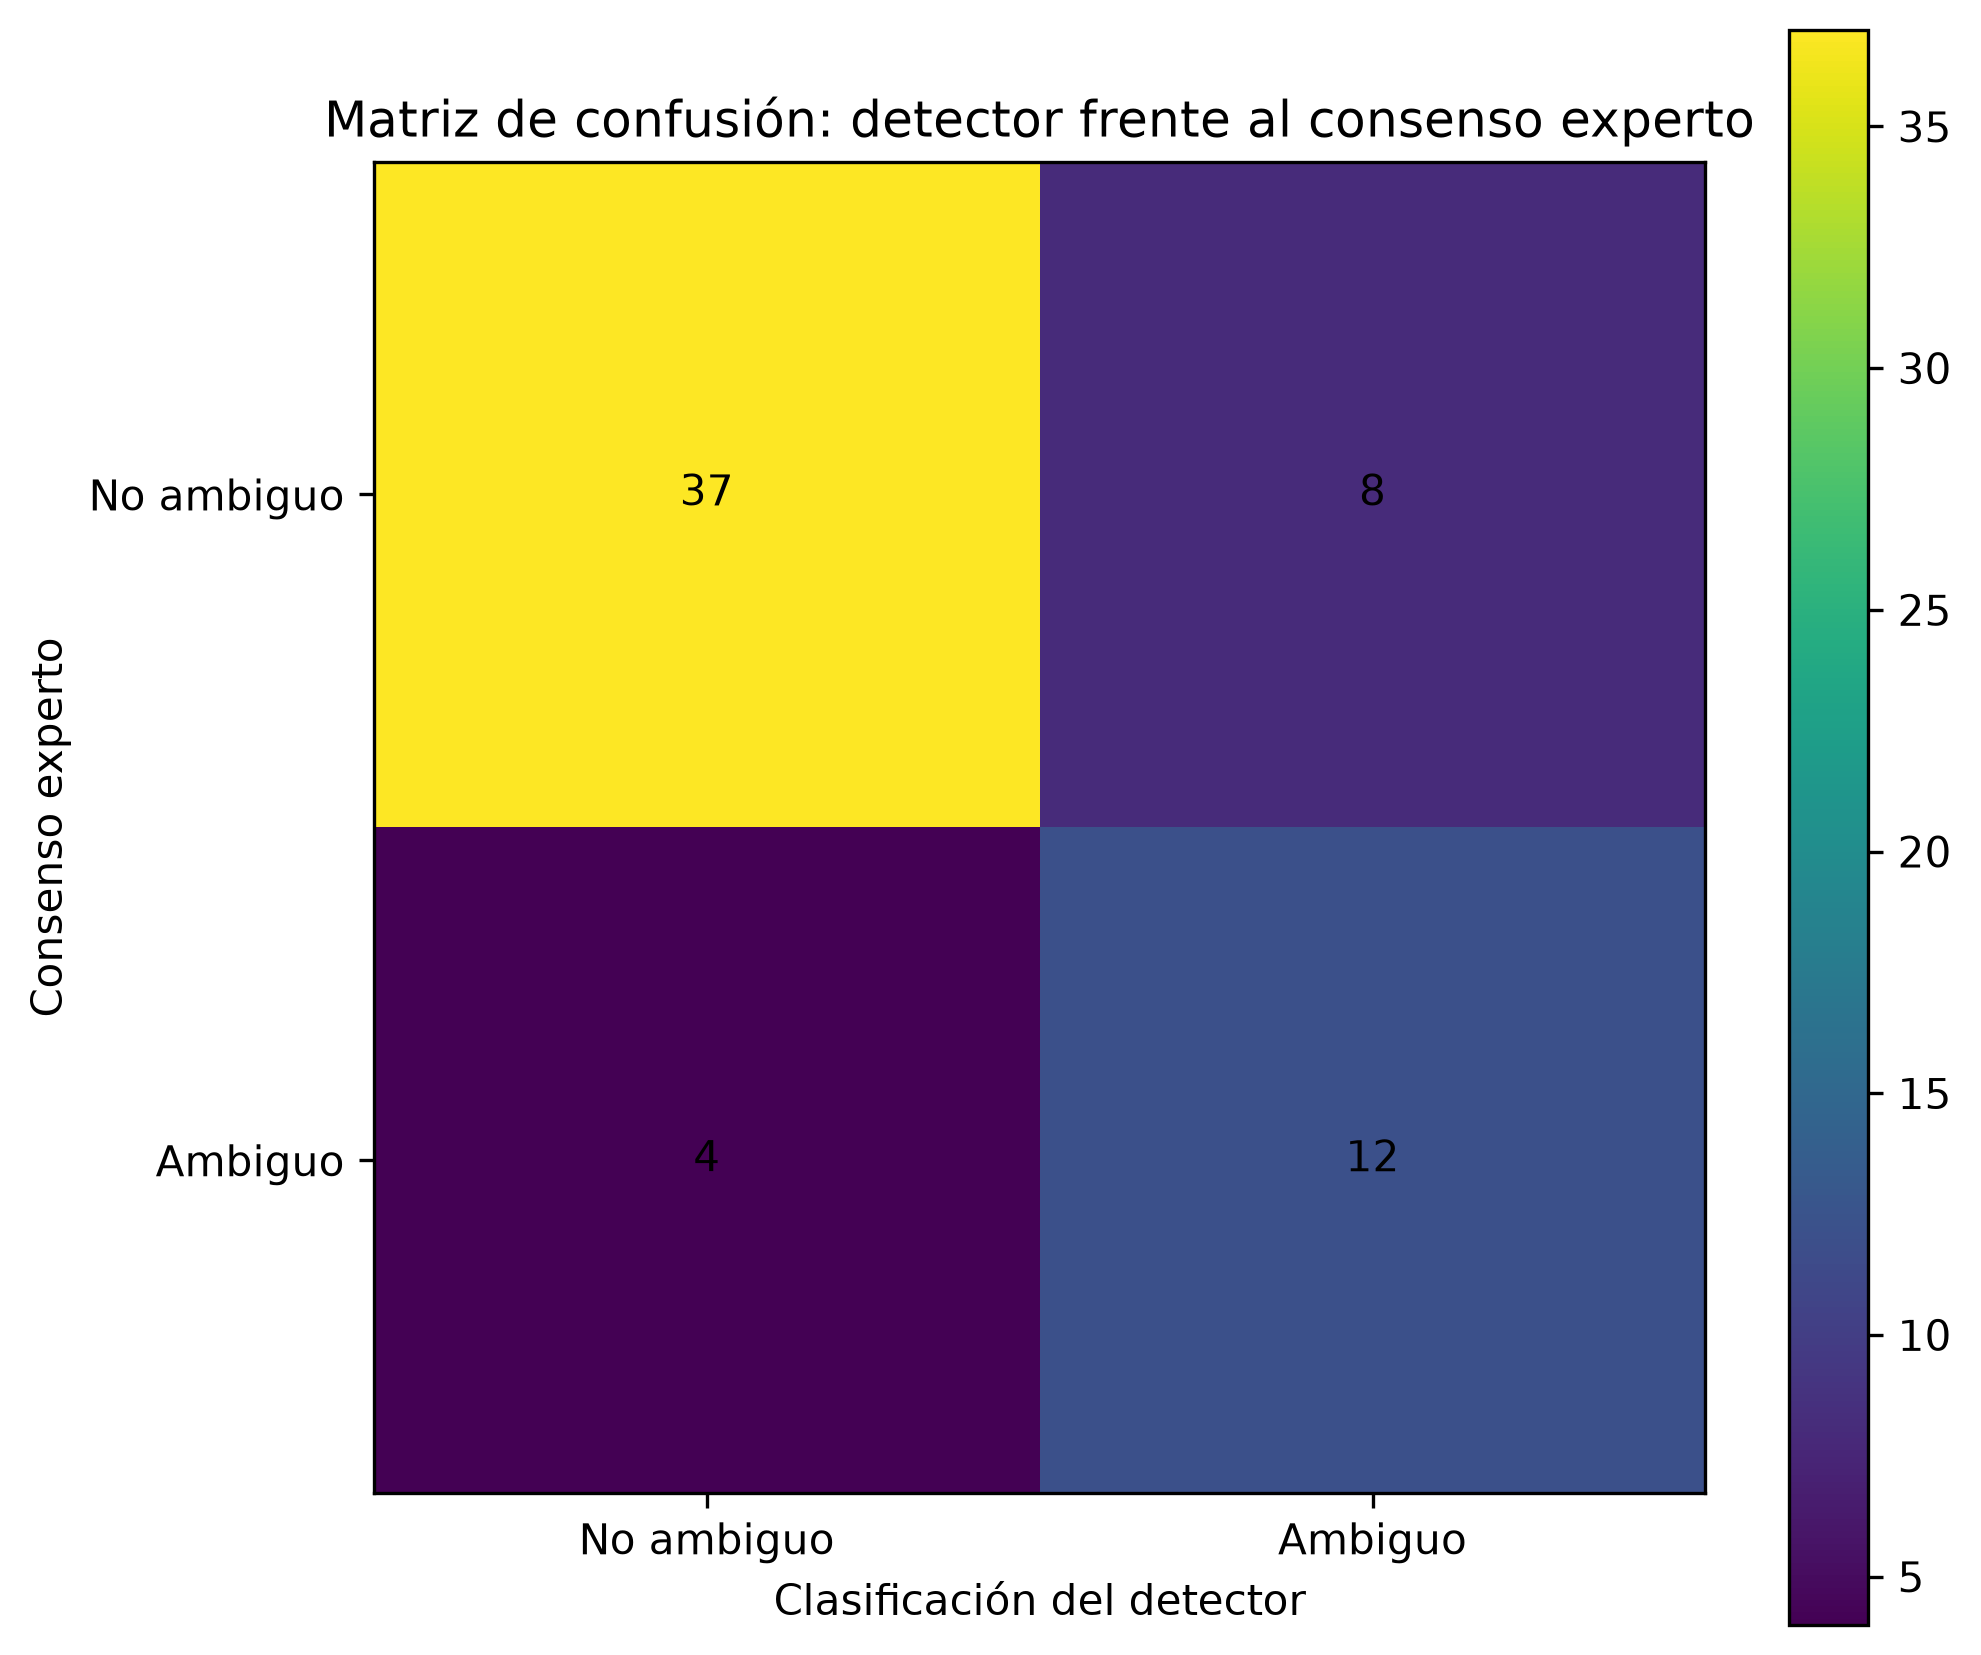
\includegraphics[width=0.7\textwidth]{figuras/figura_2_matriz_confusion.png}
		\caption{Confusion matrix: automatic detector versus expert consensus.}\label{fig:confusion}
	\end{figure}
	
	The pair of hypotheses stated in Section~\ref{subsec:hypotheses} was tested with
	a chi-squared test of independence (Pearson, with continuity correction) on the
	2$\times$2 contingency table of Figure~\ref{fig:confusion}: $\chi^2(1,
	N=61)=15.037$, $p=0.0001$, $\phi=0.497$ (Table~\ref{tab:significancia}). The
	test rejects $H_0$: the association between detector output and expert
	consensus is statistically significant and the effect size ($\phi=0.497$) is
	of medium-to-large magnitude by conventional benchmarks. The 95\% confidence
	interval for $\kappa$ ([0.280, 0.737]) excludes zero, consistent with the
	significant chi-squared result, and spans from fair to substantial agreement,
	which reflects genuine uncertainty about the precise population value at this
	sample size rather than any doubt about whether an association exists.
	
	\begin{table}[h]
		\caption{Hypothesis test and effect size for RQ1 ($H_0$/$H_1$)}\label{tab:significancia}
		\begin{tabular}{@{}ll@{}}
			\toprule
			Element & Value \\
			\midrule
			Test & Chi-squared test of independence (Pearson, continuity correction) \\
			Statistic ($\chi^2$) & 15.0374 (d.f.\ = 1) \\
			$p$ value & 0.0001 \\
			Effect size ($\phi$) & 0.4965 \\
			\botrule
		\end{tabular}
	\end{table}
	
	This significant result is strengthened, not undermined, by the reliability of
	the reference standard it is compared with. Table~\ref{tab:acuerdo-interevaluador}
	reports pairwise Cohen's $\kappa$ between experts and Fleiss' $\kappa$ across the
	full panel: the three experts agreed with each other substantially to almost
	perfectly (pairwise $\kappa$ between 0.786 and 0.919; Fleiss' $\kappa = 0.857$,
	94.54\% observed agreement). Because the panel that produced the reference
	consensus agreed with itself almost perfectly, the moderate detector-consensus
	agreement ($\kappa=0.530$) represents a genuine, well-grounded signal rather
	than an artefact of an unreliable or arbitrary reference standard.
	
	\begin{table}[h]
		\caption{Inter-rater agreement among the three experts}\label{tab:acuerdo-interevaluador}
		\begin{tabular}{@{}lrrl@{}}
			\toprule
			Comparison & Cohen's/Fleiss' $\kappa$ & Observed agreement & Interpretation \\
			\midrule
			Expert 1 vs.\ Expert 2 & 0.8647 & 0.9508 & Almost perfect \\
			Expert 1 vs.\ Expert 3 & 0.9186 & 0.9672 & Almost perfect \\
			Expert 2 vs.\ Expert 3 & 0.7857 & 0.9180 & Substantial \\
			Full panel (Fleiss' $\kappa$) & 0.8569 & 0.9454 & Almost perfect \\
			\botrule
		\end{tabular}
	\end{table}
	
	Figure~\ref{fig:kappa} plots the four agreement coefficients of
	Table~\ref{tab:acuerdo-interevaluador} against the single detector-consensus
	coefficient of Table~\ref{tab:metricas-detector}, visualising the gap between
	human--human agreement and detector--human agreement: both are high, but
	human--human agreement remains higher.
	
	\begin{figure}[h]
		\centering
		
\includegraphics[width=0.8\textwidth]{figuras/figura_3_coeficientes_kappa.png}
		\caption{Kappa coefficients: inter-expert agreement versus detector-consensus agreement.}\label{fig:kappa}
	\end{figure}
	
	Disaggregating coincidence between detector and consensus by requirement type
	(computed directly from the requirement-level table released in the replication
	package) shows a clear gradient: the detector agreed with the panel on all 9
	legal requirements (100\%), on 14 of 16 non-functional requirements (87.5\%),
	on 21 of 27 functional requirements (77.8\%), and on only 5 of 9 design
	constraints (55.6\%) (Table~\ref{tab:coincidencia-tipo}). Design constraints are
	where the detector's four lexical-syntactic rules diverge most from expert
	judgement; the sample size per stratum is too small for a separate significance
	test, but the gradient is consistent with the disagreement analysis in
	Section~\ref{subsec:res-rq2}.
	
	\begin{table}[h]
		\caption{Detector-consensus coincidence by requirement type}\label{tab:coincidencia-tipo}
		\begin{tabular}{@{}lrrr@{}}
			\toprule
			Type & $N$ & Coincides ($n$) & Coincides (\%) \\
			\midrule
			Legal requirements (RL) & 9 & 9 & 100.0 \\
			Non-functional requirements (NFR) & 16 & 14 & 87.5 \\
			Functional requirements (FR) & 27 & 21 & 77.8 \\
			Design constraints (DC) & 9 & 5 & 55.6 \\
			\botrule
		\end{tabular}
	\end{table}
	
	The full requirement-by-requirement classification table (61 rows, anonymous
	identifiers, both classifications, the rule fired, and the confidence reported
	by each expert) is released in the replication package and is not reproduced in
	full here for space; illustrative disagreement cases are discussed in
	Section~\ref{subsec:res-rq2}.
	
	\subsection{RQ2: disagreement patterns}\label{subsec:res-rq2}
	
	Table~\ref{tab:tipos-ambiguedad} reports the type of smell the three experts
	attributed to their own ambiguity markings, using the rubric's smell-type field
	recorded alongside each classification, aggregated across the 47 individual
	ambiguous markings made by the three raters (16 + 13 + 18, from
	Table~\ref{tab:resumen-clasificaciones}). Imprecise terminology is the smell
	experts cite most often (38.30\%, 18/47), followed by vague quantifier
	(31.91\%), non-verifiable or incomplete requirement (19.15\%) and, least
	frequently, multiple conjunctions concealing more than one requirement in a
	single statement (10.64\%).
	
	\begin{table}[h]
		\caption{Types of ambiguity experts attributed to their own markings}\label{tab:tipos-ambiguedad}
		\begin{tabular}{@{}lrr@{}}
			\toprule
			Type of ambiguity & Frequency & \% of ambiguous markings \\
			\midrule
			Imprecise terminology & 18 & 38.30 \\
			Vague quantifier & 15 & 31.91 \\
			Non-verifiable / incomplete requirement & 9 & 19.15 \\
			Multiple conjunction & 5 & 10.64 \\
			\botrule
		\end{tabular}
	\end{table}
	
	\begin{figure}[h]
		\centering
		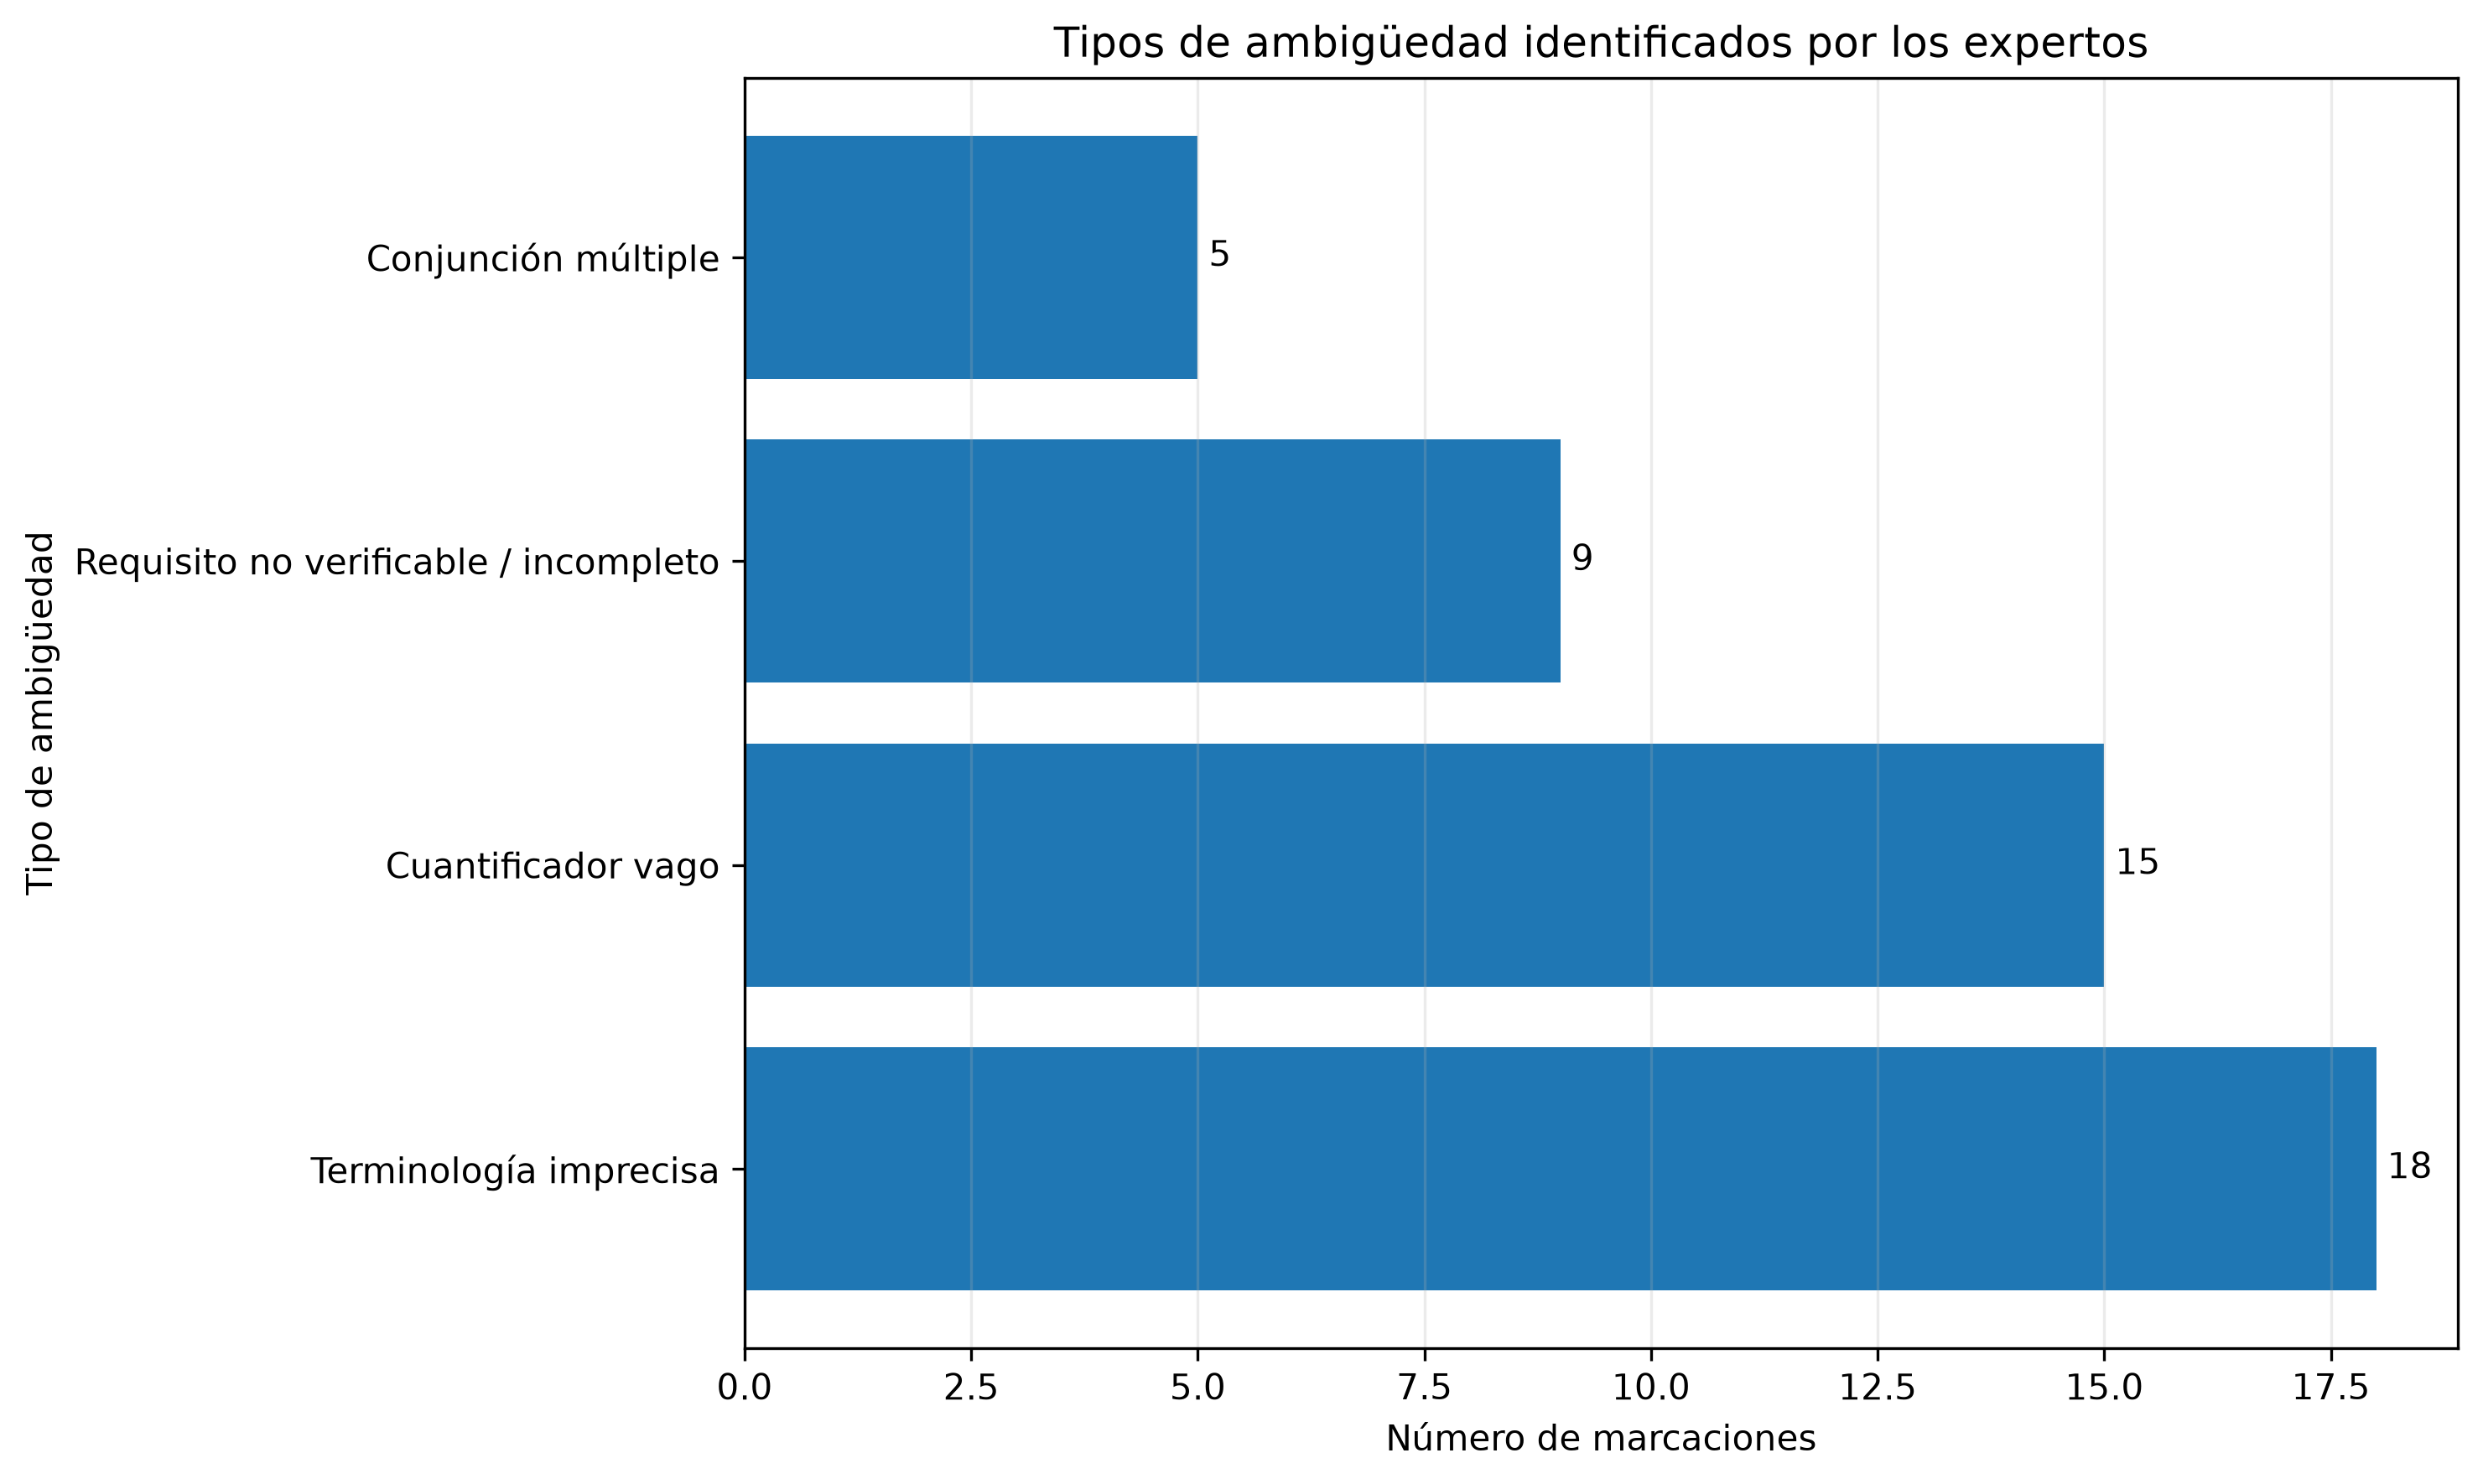
\includegraphics[width=0.8\textwidth]{figuras/figura_4_tipos_ambiguedad.png}
		\caption{Types of ambiguity attributed by experts to their flagged requirements.}\label{fig:tipos}
	\end{figure}
	
	The detector's own rule log, read against the 20 requirements it flagged as
	ambiguous, shows a comparatively even spread across four labels tailored to
	requirement type: imprecise terminology / lack of verifiability (8 firings,
	mostly on functional requirements), imprecise regulatory terminology (5
	firings, exclusively on legal requirements), incomplete design constraint (4
	firings, exclusively on design constraints) and vague quantifier / insufficient
	threshold (3 firings). No requirement in this corpus triggered more than one
	rule.
	
	Two disagreement patterns account for the 12 requirements where detector and
	consensus diverge (Figure~\ref{fig:confusion}, off-diagonal cells). The larger
	pattern (8 cases, false positives) is the detector over-flagging requirements
	the panel judged non-ambiguous, concentrated in the ``imprecise terminology /
	verifiability'' rule: for example REQ-53 (RNF-04, a usability requirement)
	states that ``at least 90\% of users complete the main tasks $\ldots$ without
	prior training, and reach a mean System Usability Scale score $\geq 80/100$''
	--- a requirement with two explicit numeric thresholds --- yet triggered the
	detector's vague-quantifier rule, which the panel unanimously judged
	non-ambiguous (3/3). REQ-08 (RF-12, identity verification via an official
	document) and REQ-24 (RF-11, owner-controlled visibility of sensitive pet and
	profile data) show the same pattern: both triggered the imprecise-terminology
	rule, and both were unanimously judged non-ambiguous by the panel, because the
	verification procedure the rule looks for (an explicit numeric or testable
	threshold in the sentence itself) is not what the three experts required to
	consider a requirement verifiable in practice --- checking that an uploaded
	document is valid, or that a visibility toggle exists, does not need a stated
	number to be testable. The smaller pattern (4 cases, false negatives) is the
	detector missing requirements the panel judged ambiguous, three of them
	unanimously: REQ-18 (RD-04, protecting personal and clinical data ``by design
	and by default'' per Art.\ 39 LOPDP, triggering no rule at all) and REQ-42
	(RF-08, a cross-breeding request accepted or rejected ``based on the available
	information'', also triggering no rule) both contain no vague quantifier,
	multiple conjunction, or the specific verification-criterion pattern the rules
	look for, yet the panel considered both under-specified --- neither states
	\emph{which} mechanism or \emph{which} information, a pragmatic gap the current
	rule set has no mechanism to represent. REQ-56 (RF-26, a second veterinarian
	confirming or questioning a prior medical validation) was the sole false
	negative with a split panel vote (2/3), the only disagreement case in this
	corpus where the experts themselves were not unanimous.
	
	The secondary analysis planned in Section~\ref{subsec:analysis} asked whether
	the requirements where detector and consensus disagree are also the ones where
	experts reported lower confidence in their own judgement --- which would suggest
	the detector fails specifically on genuinely hard cases. The mean confidence
	reported per requirement (average across the three experts, 1--5 scale) did not
	follow a normal distribution (Shapiro--Wilk $W=0.699$, $p<0.001$), so the
	Mann--Whitney $U$ test was used. Mean confidence was similar between the 49
	requirements where detector and consensus coincide ($M=4.54$, $SD=0.51$) and
	the 12 where they disagree ($M=4.39$, $SD=0.65$); the difference is not
	significant ($U=350.0$, $p=0.257$, Cliff's $\delta=0.191$, negligible-to-small,
	Table~\ref{tab:confianza}). Experts were not meaningfully less confident on the
	requirements where the detector disagreed with them, which indicates the
	detector's errors are not concentrated on the panel's own hardest,
	lowest-confidence borderline cases, but reflect a specific mismatch between the
	rule set and the design-constraint/verification-procedure judgements the panel
	makes confidently.
	
	\begin{table}[h]
		\caption{Secondary analysis: expert confidence vs.\ detector-consensus coincidence}\label{tab:confianza}
		\begin{tabular}{@{}lrl@{}}
			\toprule
			Element & Value & Detail \\
			\midrule
			Shapiro--Wilk (mean confidence, $N=61$) & $W=0.6994$ & $p<0.0001$ (rejects normality) \\
			Coincides ($n=49$) & $M=4.5442$ & $SD=0.5123$ \\
			Disagrees ($n=12$) & $M=4.3889$ & $SD=0.6487$ \\
			Mann--Whitney $U$ & 350.00 & $N=61$ \\
			$p$ value & 0.2566 & --- \\
			Cliff's $\delta$ & 0.1905 & negligible-to-small \\
			\botrule
		\end{tabular}
	\end{table}
	
	%=====================================================================
	% --- Sección a cargo de: Morales Sánchez, G. A. (Documentador) ---
	\section{Discussion}\label{sec:discussion}
	
	\subsection{Implications for research}\label{subsec:disc-research}
	
	The central finding --- moderate, statistically significant agreement between a
	four-rule lexical-syntactic detector and an almost-perfectly agreeing expert
	panel ($\kappa=0.530$ vs.\ $\kappa=0.857$, Tables~\ref{tab:metricas-detector}
	and~\ref{tab:acuerdo-interevaluador}) --- qualifies rather than contradicts the
	concern raised by Ferrari et al.~\cite{ferrari2016} that ambiguity in
	requirements is entangled with tacit knowledge a purely lexical approach cannot
	access. That concern holds, but unevenly: the type-level breakdown
	(Table~\ref{tab:coincidencia-tipo}) shows the detector reaches perfect
	agreement on legal requirements and near-ceiling agreement on non-functional
	requirements, and only degrades sharply on design constraints (55.6\%). The
	research implication is therefore not that lexical detection has a uniform
	ceiling, but that the ceiling is type-dependent: requirement types whose
	ambiguity tends to hinge on an explicit, checkable element (a numeric
	threshold, a named legal article, a stated actor) are more tractable for a
	rule-based approach than requirement types --- design constraints in this
	corpus --- whose ambiguity more often lies in an unstated mechanism or
	procedure.
	
	The false-positive analysis in Section~\ref{subsec:res-rq2} narrows this
	further. REQ-53 is the clearest case: it contains \emph{two} explicit numeric
	thresholds (90\% of users, SUS $\geq 80/100$) and was still flagged by the
	vague-quantifier rule, which the panel unanimously rejected. This is not
	evidence that vague-quantifier detection is unreliable in general; it is
	evidence that the specific rule implementation reacts to a lexical trigger
	(phrases such as ``at least'') without checking whether a concrete number
	already follows it. This is a narrower, more actionable finding than ``lexical
	rules miss context'': it identifies a fixable pattern-matching gap in one rule,
	rather than a general limitation of the rule-based paradigm.
	
	The false negatives point in a different, complementary direction. REQ-18 and
	REQ-42 --- both unanimously judged ambiguous by the panel, both triggering no
	rule at all --- share an absence of a stated \emph{mechanism} or
	\emph{referent} (``mediante mecanismos de autenticación y autorización''
	without specifying which; ``con base en la información disponible'' without
	specifying which information). None of the four current rules targets
	underspecified mechanism references, which is a plausible explanation for why
	design constraints --- a requirement type that by definition describes
	constraints on \emph{how} something is implemented --- are where the detector's
	recall is weakest.
	
	The null result of the secondary analysis (Table~\ref{tab:confianza}, $p=0.257$)
	is itself a research-relevant finding: it rules out the more comfortable
	explanation that the detector simply struggles on the panel's own
	low-confidence, genuinely hard cases. Experts were confidently unanimous on
	several of the cases the detector got wrong (REQ-18, REQ-42, REQ-53 all 3/3).
	The detector's errors are therefore a mismatch of what counts as evidence of
	ambiguity, not a difficulty concentrated where human judgement is itself
	uncertain --- which is the more tractable finding for future rule design to act
	on.
	
	\subsection{Implications for practice}\label{subsec:disc-practice}
	
	For a practitioner deciding whether to adopt this detector as a review gate for
	a real specification like MundiPets, these results support a qualified
	recommendation the earlier, smaller pilot could not: at accuracy = 0.803 and a
	statistically significant, moderate agreement with an almost-perfectly
	agreeing expert panel, the detector is a credible first-pass triage tool for
	functional, non-functional and, especially, legal requirements, where it
	reached perfect agreement on this corpus. It would meaningfully reduce reviewer
	workload without discarding real ambiguity: of the 45 requirements the panel
	judged non-ambiguous, it correctly cleared 37 (82.2\% specificity), and of the
	16 the panel judged ambiguous, it correctly caught 12 (75.0\% recall).
	
	The practical caveat is equally clear from the data: design constraints are the
	one requirement type where this detector should not be trusted unsupervised.
	Its coincidence with the panel drops to 55.6\% there, barely above chance for a
	binary label, and the two clearest false negatives in the entire corpus (REQ-18
	and REQ-42) both fall in that category, one of them directly tied to a legal
	data-protection obligation (Art.\ 39 LOPDP). For a system like MundiPets that
	processes personal and animal health data under Ecuador's
	LOPDP~\cite{lopdp2021}, a design constraint silently missed by an automatic
	gate is precisely the kind of ambiguity whose downstream cost is highest. The
	practical recommendation is therefore type-conditional: automate the triage of
	functional, non-functional and legal requirements, and route design
	constraints to mandatory human review regardless of what the detector reports.
	
	\subsection{Surprising or counter-intuitive findings}\label{subsec:disc-surprising}
	
	Two results ran against the team's expectation going into the analysis. First,
	the overall strength of the result: with a small, hand-written four-rule
	detector and a corpus written by novice analysts, the team expected agreement
	closer to what the smaller 50-item pilot of this study had shown (slight,
	non-significant) than the moderate, significant agreement the completed
	61-item corpus produced. The revision and expansion of the corpus --- driven by
	correcting the requirement numbering rather than by any change to the detector
	or the evaluation protocol --- changed the empirical picture substantially,
	which is itself a useful methodological lesson: a quasi-experiment's
	conclusions can be sensitive to corpus completeness in ways a single pilot run
	does not reveal, and a preregistered protocol with a versioned corpus and
	reproducible scripts (Section~\ref{sec:results}) is what makes that sensitivity
	visible rather than hidden.
	
	Second, the specific content of the false positives (Table~\ref{tab:confianza}
	notwithstanding) was counter-intuitive: the team expected the vague-quantifier
	rule to be the detector's most reliable rule, precisely because it targets an
	apparently unambiguous lexical pattern. Instead, REQ-53 shows that rule firing
	even on a requirement with two explicit numeric thresholds, which suggests the
	rule is keying on a trigger phrase (``al menos'') rather than verifying the
	absence of a following number --- an implementation detail invisible from the
	rule's name alone, and only surfaced by manually inspecting the disagreement
	cases rather than by trusting the aggregate metrics.
	
	
	%=====================================================================
	% --- Sección a cargo de: Gutiérrez Ortega, G. A. (Verificadora) ---
	\section{Threats to validity}\label{sec:threats}
	
	Threats are organised in the four categories of Wohlin et
	al.~\cite{wohlin2012}. For each, the anticipated threat documented in the
	preregistered OSF protocol is carried over, together with the mitigation
	applied and the limitation that remains after that mitigation.
	
	\subsection{Internal validity}\label{subsec:threats-internal}
	
	\emph{Detector-team overlap.} The same team that specified the MundiPets
	requirements also designed and froze the detector's four rules.
	\emph{Mitigation:} the detector was frozen in code before any classification
	was run, and its rules were derived from the general requirements-quality
	literature rather than tuned by inspecting the corpus; the preregistration
	timestamp on the Open Science Framework predates both the distribution of the
	rubric to the expert panel and the detector's execution over the corpus,
	precluding post-hoc adjustment. \emph{Residual limitation:} the rules were
	still authored by people familiar with the corpus's domain and writing style,
	which cannot be fully separated from having built the specification.
	
	\emph{Rater independence.} A dependent, non-blind evaluation would inflate
	agreement between raters and between raters and the detector.
	\emph{Mitigation:} the three experts were external to the MundiPets team, blind
	to the detector's output and to each other's classifications, and evaluated
	requirements presented in independently randomised order with type labels
	stripped (Section~\ref{subsec:design}). The almost-perfect inter-rater
	agreement obtained (Fleiss' $\kappa=0.857$) is evidence the blinding held.
	\emph{Residual limitation:} all three raters share the same institutional
	background (professional degree from the same university), which may correlate
	their notion of what counts as ``verifiable'' more than a panel drawn from
	different institutions would.
	
	\subsection{External validity}\label{subsec:threats-external}
	
	\emph{Single system, single domain, single language.} The corpus is the
	complete but singular specification of one social network for pet adoption and
	breeding, written in Spanish by novice analysts in an academic setting in
	Ecuador. \emph{Mitigation:} none directly available within this study; the
	replication package (detector code, corpus, expert classifications, analysis
	scripts) is released precisely so the design can be repeated on other domains,
	languages and author populations. \emph{Residual limitation:} the reported
	metrics --- particularly the strong type-dependent gradient (100\% on legal
	requirements, 55.6\% on design constraints) --- should not be extrapolated
	beyond Spanish-language specifications written by requirements-engineering
	students; whether the same gradient holds for professional analysts, other
	languages, or specifications with a different balance of requirement types is
	an open question this single study cannot answer.
	
	\emph{Requirement population size bounded by the real system, and revised
		mid-study.} $N=61$ is not a sample drawn from a larger population of MundiPets
	requirements; it is the complete population at the time of the experiment,
	after a numbering correction that expanded the corpus from an earlier
	50-requirement version. \emph{Mitigation:} because $N$ is the full population
	rather than a sample, there is no sampling bias within this system, and the
	corpus revision was a correction of requirement identifiers and completeness
	--- not a selection of favourable cases after seeing the detector's results, a
	distinction documented in the OSF deviations log
	(Section~\ref{subsec:analysis}). \emph{Residual limitation:} a corpus of 61
	items is nonetheless small relative to industrial specifications, and results
	may not generalise to specifications an order of magnitude larger, where
	different type distributions and smell patterns could dominate; the fact that
	the conclusion changed materially between the 50-item and 61-item versions of
	this corpus (Section~\ref{subsec:disc-surprising}) is itself evidence that
	conclusions at this scale remain sensitive to corpus completeness.
	
	\subsection{Construct validity}\label{subsec:threats-construct}
	
	\emph{Ambiguity operationalised as a binary label.} Both the detector and the
	expert rubric reduce ambiguity to a binary ambiguous/non-ambiguous judgement per
	requirement, discarding degree, multiplicity of smells within one requirement,
	and the specific linguistic construct involved. \emph{Mitigation:} the
	smell-type field recorded alongside every expert marking
	(Table~\ref{tab:tipos-ambiguedad}) and the detector's per-rule log partially
	recover this lost granularity and were used throughout
	Section~\ref{subsec:res-rq2} to characterise \emph{how}, not just \emph{whether},
	detector and experts disagree. \emph{Residual limitation:} the primary
	hypothesis test (Table~\ref{tab:significancia}) is still computed on the binary
	collapse, which may understate agreement on requirements where detector and
	experts identify the same underlying smell but the detector's binary output
	happens to fall on the wrong side of the threshold.
	
	\emph{Consensus by majority vote as ground truth.} Expert consensus was defined
	as majority vote across three raters (Section~\ref{subsec:analysis}), which
	treats disagreement among experts as resolved rather than as informative.
	\emph{Mitigation:} pairwise and full-panel agreement are reported separately
	(Table~\ref{tab:acuerdo-interevaluador}) precisely so a reader can assess how
	much the majority-vote collapse could be masking; with Fleiss' $\kappa=0.857$
	for the full panel, the collapse discards comparatively little information.
	\emph{Residual limitation:} the single case decided 2/3 rather than 3/3 in this
	corpus (REQ-56, Section~\ref{subsec:res-rq2}) still enters the primary analysis
	with the same weight as unanimous cases, which a more conservative design might
	have excluded or weighted differently.
	
	\subsection{Conclusion validity}\label{subsec:threats-conclusion}
	
	\emph{Statistical power.} The chi-squared test in
	Section~\ref{subsec:res-rq1} is significant ($p=0.0001$) at $N=61$, and the
	95\% confidence interval for $\kappa$ ([0.280, 0.737], Table~\ref{tab:metricas-detector})
	excludes zero, which gives reasonable confidence that a real association
	exists. \emph{Mitigation:} because $N$ is fixed by the size of the real,
	completed specification rather than by an expandable recruitment target
	(Section~\ref{subsec:analysis}), the study reports the full confidence
	interval rather than the point estimate alone; the interval is still wide
	enough (0.280 to 0.737) to span fair through substantial agreement, and the
	per-type breakdown (Table~\ref{tab:coincidencia-tipo}) is explicitly reported
	as descriptive rather than separately tested, given the small stratum sizes
	(as few as 9 items per type). \emph{Residual limitation:} the study cannot, at
	this sample size, distinguish precisely how much of the observed $\kappa=0.530$
	is driven by the near-ceiling performance on legal and non-functional
	requirements versus the weaker performance on design constraints; a
	type-stratified analysis with a larger corpus would be needed to test the
	type gradient formally rather than describe it.
	
	\emph{Reliability of the automated computations.} Manual computation of
	agreement coefficients, bootstrap intervals and hypothesis tests is error-prone
	and difficult to audit. \emph{Mitigation:} every value in
	Section~\ref{sec:results} is produced by versioned Python scripts
	(\texttt{06\_Experimento/scripts\_analisis/}) executed end to end through a
	single entry point (\texttt{run\_all.py}) over the raw detector output and
	expert classifications released in the replication package; no figure or table
	was produced or edited by hand, and the full pipeline was re-executed after the
	corpus revision to regenerate every number in this manuscript from the
	corrected raw data. \emph{Residual limitation:} correctness of the underlying
	formulas (e.g.\ the closed-form expression used for Cohen's $\kappa$) was
	checked against the standard definitions in Cohen~\cite{cohen1960} and
	Fleiss~\cite{fleiss1971} but not against an independent second implementation,
	which a stricter reproducibility standard would require.
	
	
	%=====================================================================
	% --- Sección a cargo de: Nieves Sánchez, J. S. (Verificador) ---
	\section{Conclusions and future work}\label{sec:conclusions}
	
	\textbf{RQ1.} With what precision, recall and $F_1$ does a rule-based automatic
	detector replicate the consensus judgement of human experts when classifying
	the requirements of MundiPets as ambiguous? The detector reached accuracy =
	0.803, precision = 0.600, recall = 0.750 and $F_1 = 0.667$ against expert
	consensus, with agreement that was moderate (Cohen's $\kappa=0.530$) and
	statistically significant at $N=61$ ($\chi^2=15.037$, $p=0.0001$). This
	result is strengthened by the reliability of the reference standard: the same
	three experts agreed with each other almost perfectly (Fleiss' $\kappa=0.857$).
	The answer to RQ1 is that, on this corpus, a four-rule lexical-syntactic
	detector achieves a real, statistically defensible level of agreement with
	expert consensus, but that agreement is strongly type-dependent: perfect on
	legal requirements (100\%), high on non-functional requirements (87.5\%), good
	on functional requirements (77.8\%), and considerably weaker on design
	constraints (55.6\%).
	
	\textbf{RQ2.} Which disagreement patterns predominate between the automatic
	detector and expert judgement, and what do they reveal about the limits of a
	rule-based approach relative to human judgement in identifying ambiguity? Two
	patterns predominate among the 12 disagreements. The false-positive pattern (8
	cases) is driven by rules that fire on a lexical trigger without checking
	whether the sentence already contains the precise information the trigger is
	meant to flag as missing --- most clearly illustrated by a usability
	requirement with two explicit numeric thresholds that still triggered the
	vague-quantifier rule. The false-negative pattern (4 cases) is driven by
	requirements whose ambiguity lies in an unstated mechanism or referent (``by
	means of authentication and authorisation mechanisms'', unspecified;
	``based on the available information'', unspecified), a pragmatic gap none of
	the four rules targets, and which concentrates disproportionately in design
	constraints. Expert confidence did not differ between the two groups
	(Mann--Whitney $U=350.0$, $p=0.257$), indicating these disagreements are not
	concentrated on the panel's own hardest, lowest-confidence cases, but reflect a
	specific, identifiable mismatch between what the rule set operationalises and
	what experts require for a requirement to count as unambiguous.
	
	Consolidating the three contributions promised in Section~\ref{sec:intro}: this
	study delivers (i) a quantified, statistically tested comparison between a
	frozen rule-based detector and a blind three-expert consensus over a complete,
	real, Spanish-language requirements corpus spanning four requirement types,
	with agreement metrics, confidence intervals and a formal hypothesis test that
	establishes a statistically significant, moderate level of agreement; (ii) a
	per-rule, per-type characterisation of where and why detector and human
	judgement diverge, identifying a fixable pattern-matching gap in the
	vague-quantifier rule and a systematic recall gap on design constraints driven
	by unstated mechanisms rather than by ambiguity in general; and (iii) a
	complete replication package --- corpus, detector code, individual and
	consensus expert classifications, analysis scripts and the preregistered
	protocol --- released under CC~BY~4.0, so that every number in
	Section~\ref{sec:results} can be regenerated and the design repeated on other
	corpora.
	
	Three concrete lines of future work follow directly from the data reported
	here. First, fix the vague-quantifier rule to check for an already-present
	numeric threshold before flagging a requirement, using REQ-53 as a concrete
	regression test case, and re-run the same protocol on the same corpus to
	measure whether precision improves without a proportional loss in recall.
	Second, add a rule targeting underspecified mechanism or method references
	(the pattern behind the false negatives identified in
	Section~\ref{subsec:res-rq2}), specifically tuned to design constraints, where
	recall is weakest (55.6\% coincidence), and evaluate whether it closes that
	gap without degrading the near-perfect performance already achieved on legal
	and non-functional requirements. Third, repeat this exact design --- frozen
	detector, blind three-expert panel, preregistered protocol, open replication
	package --- on a specification of comparable size and comparable type
	distribution from a different domain and, ideally, a different institution, to
	test whether the type-dependent gradient reported here (strong on legal and
	non-functional requirements, weak on design constraints) is a property of this
	detector and this corpus or a more general pattern in rule-based ambiguity
	detection for Spanish-language requirements.
	
	%=====================================================================
	\backmatter
	
	\bmhead{Acknowledgements}
	
	The authors thank the three software engineers who served as expert raters and
	the veterinary practice in Quevedo, Ecuador, that granted access to its
	operational context and which remains pseudonymised under the anonymisation
	protocol of this study.
	
	% --- Sección a cargo de: Nieves Sánchez, J. S. (Verificador) ---
	\section*{Declarations}
	
	\begin{itemize}
		\item \textbf{Funding.} This research received no specific grant from any
		funding agency in the public, commercial or not-for-profit sectors.
		\item \textbf{Competing interests.} The authors declare no competing interests.
		\item \textbf{Ethics approval and consent to participate.} The study was
		conducted under the ethics framework of the Requirements Engineering course at
		the Universidad Técnica Estatal de Quevedo. All participants signed an informed
		consent form drafted in compliance with Ecuador's Organic Law on Personal Data
		Protection~\cite{lopdp2021}.
		\item \textbf{Consent for publication.} All participants explicitly authorised
		the use of their anonymised data in peer-reviewed publications and its deposit
		in an open dataset.
		\item \textbf{Data availability.} The preregistered protocol is available on the
		Open Science Framework at https://osf.io/khyf2/overview, registered on 27 July
		2026 at 10:49:41 (Ecuador time), before data collection began. The anonymised
		dataset --- labelled requirements corpus, detector output, individual and
		consensus expert classifications, traceability matrix and analysis scripts ---
		is deposited on Zenodo under a CC~BY~4.0 licence, DOI
		10.5281/zenodo.22218780 (https://doi.org/10.5281/zenodo.22218780), following
		the FAIR principles~\cite{wilkinson2016} and the software citation principles
		of Smith et al.~\cite{smith2016}.
		\item \textbf{Materials availability.} Not applicable.
		\item \textbf{Code availability.} The detector and the analysis scripts are
		available in the project repository at
		https://github.com/andymendozap03/MundiPets-PFC-IngReq, and in the Zenodo
		deposit above.
		\item \textbf{Use of AI-assisted technologies.} The authors used Claude Opus 5
		and Claude Sonnet 5 (Anthropic) exclusively to review previously drafted text:
		checking grammar, clarity and register of paragraphs the authors had already
		written from their own empirical data and analysis. No content was drafted,
		generated or substantively rewritten by these tools; every claim, number,
		interpretation and conclusion originates from the authors' own analysis of the
		data described in Section~\ref{sec:method} and reported in
		Section~\ref{sec:results}. This is consistent with Springer Nature's editorial
		policy on artificial intelligence~\cite{springer2023}, under which AI tools may
		assist with language editing of author-written content but may not be listed as
		authors and may not generate original research content. Under no circumstance
		was an LLM used to produce results, figures, tables or conclusions: every
		quantitative claim in Section~\ref{sec:results} is generated by the versioned
		scripts in 06\_Experimento/scripts\_analisis/ from the raw detector output and
		expert classifications, as required by the course's integrity policy.
		\item \textbf{Author contribution.} E.D.F.A.: conceptualization,
		investigation, writing --- original draft. G.A.G.O.: software (design and
		implementation of the rule-based detector). A.J.M.P.: methodology,
		visualization (system modelling and diagrams). G.A.M.S.: investigation, data
		curation (interviews and transcriptions). J.S.N.S.: formal analysis, data
		curation, project administration (protocol preregistration and statistical
		analysis). G.C.G.U.: supervision, validation. All authors reviewed and approved
		the final manuscript.
	\end{itemize}
	
	%=====================================================================
	\bibliography{referencias}
	
\end{document}
